\section{Análise no Tempo Contínuo}

\subsection{Representação em Espaço de Estados}

O modelo não linear foi linearizado por expansão em série de Taylor de primeira ordem em torno do ponto de operação em regime estacionário apresentado no Apêndice~\ref{sec:apendice_ponto_operacao}.
Em termos das variáveis de desvio, o modelo linearizado assume a forma de espaço de estados
\begin{align}
  \dot{\mathbf{x}}(t) & = \mathbf{A}\,\mathbf{x}(t) + \mathbf{B}\,\mathbf{u}(t), \\
  \mathbf{y}(t)       & = \mathbf{C}\,\mathbf{x}(t),
\end{align}
em que $\mathbf{x}(t) \in \mathbb{R}^{9}$ é o vetor de estados, $\mathbf{u}(t) \in \mathbb{R}^{3}$ é o vetor de entradas e $\mathbf{y}(t) \in \mathbb{R}^{9}$ é o vetor de saídas, todos em desvio em relação ao ponto de operação.
As matrizes $\mathbf{A} \in \mathbb{R}^{9 \times 9}$, $\mathbf{B} \in \mathbb{R}^{9 \times 3}$ e $\mathbf{C} \in \mathbb{R}^{9 \times 9}$ são, respectivamente, as matrizes de estado, de entrada e de saída.

As entradas do sistema são as vazões de alimentação e de reciclo,
\begin{equation}
  \mathbf{u} = \begin{bmatrix} F_{f1} & F_{f2} & F_R \end{bmatrix}^\top,
\end{equation}
e os estados são as temperaturas e as frações molares dos componentes $A$ e $B$ nas três unidades,
\begin{equation}
  \mathbf{x} = \begin{bmatrix} T_1 & T_2 & T_3 & x_{A1} & x_{B1} & x_{A2} & x_{B2} & x_{A3} & x_{B3} \end{bmatrix}^\top.
\end{equation}

Como todos os estados são tomados como saídas, tem-se $\mathbf{y} = \mathbf{x}$ e, portanto, $\mathbf{C} = \mathbf{I}_{9}$, a matriz identidade de ordem 9.
As matrizes $\mathbf{A}$, $\mathbf{B}$ e $\mathbf{C}$ completas são apresentadas no Apêndice~\ref{sec:apendice_ABC}.

A Figura~\ref{fig:lin_vs_nlin} compara as respostas dos modelos linear e não linear de $x_{B1}$ a degraus em $F_{f1}$.
Para a perturbação pequena, o modelo linearizado reproduz bem o comportamento não linear, o que confirma sua validade na vizinhança do ponto de operação.
À medida que a perturbação se afasta do ponto de operação, porém, os modelos divergem, e o modelo linear chega a prever uma fração molar negativa, sem significado físico.
Ao retornar ao valor nominal, as respostas voltam a coincidir.
Assim, o modelo linearizado é adequado apenas para pequenas variações em torno do ponto de operação.

\begin{figure}[ht]
  \centering
  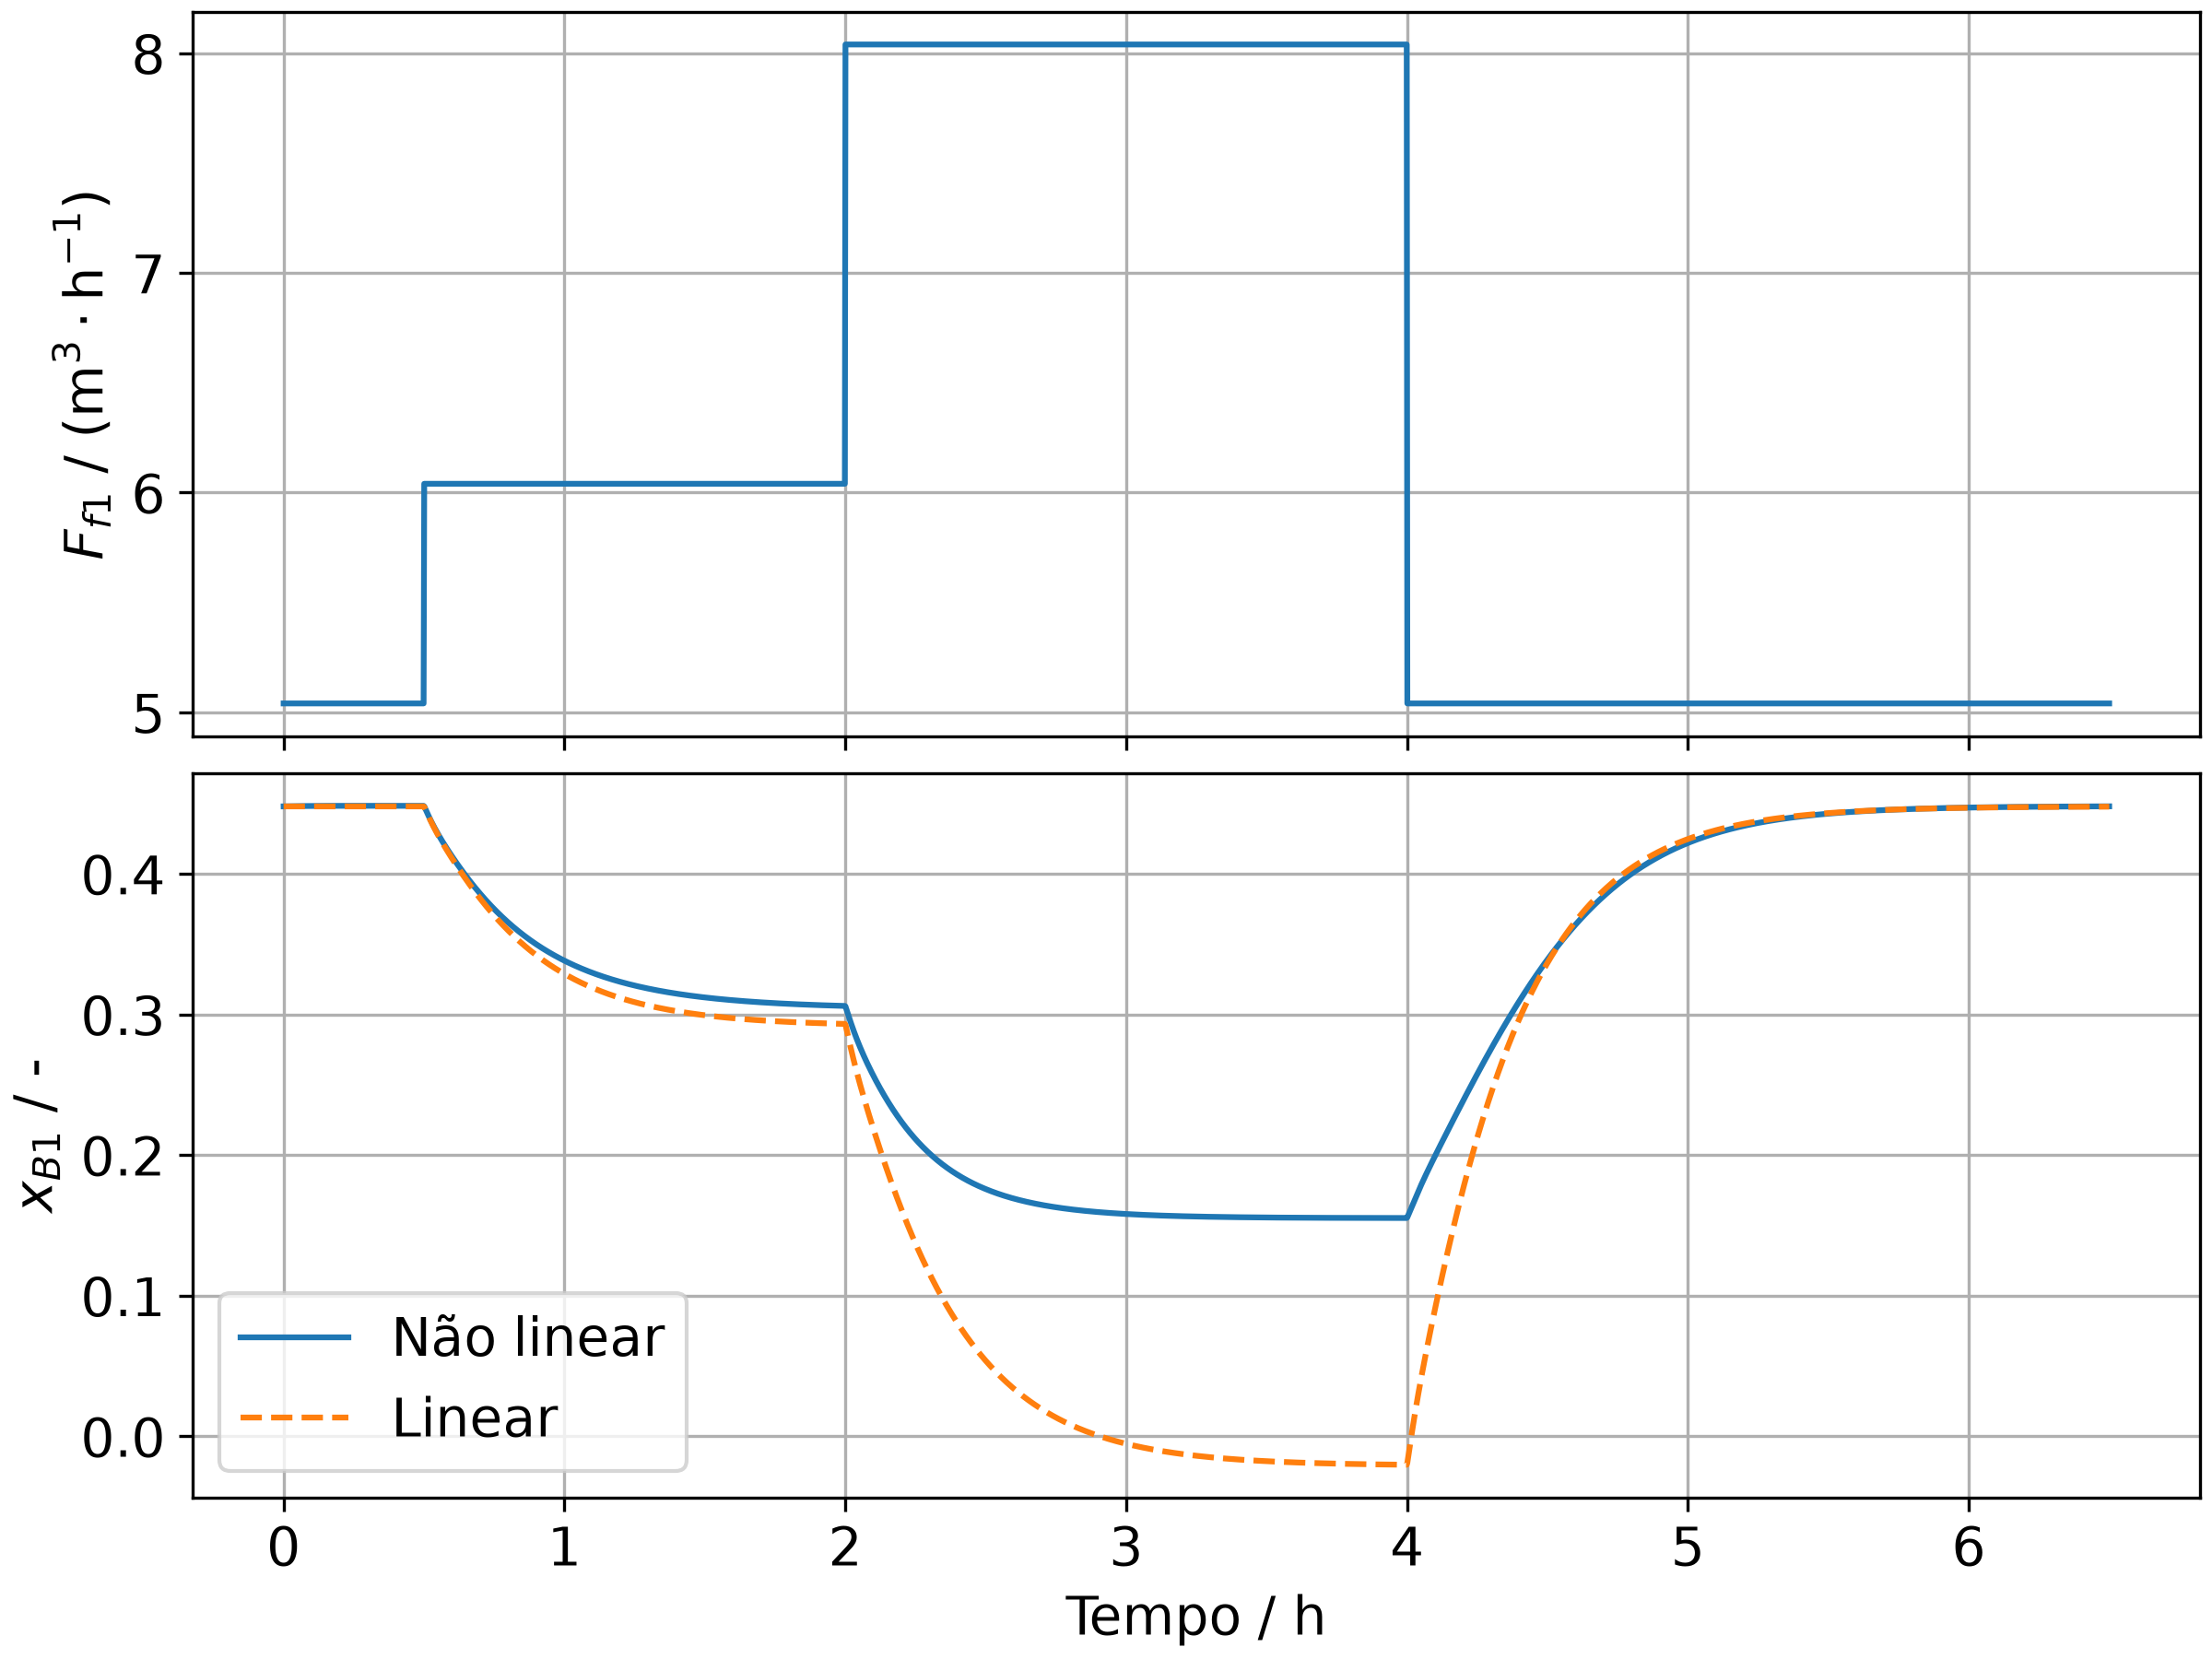
\includegraphics[width=0.6\textwidth]{../../figures/linear_vs_nonlinear/xB1_Ff1.png}
  \caption{Comparação entre as respostas dos modelos linear e não linear da fração molar $x_{B1}$ a degraus na vazão de alimentação $F_{f1}$: entrada (acima) e saída (abaixo).}
  \label{fig:lin_vs_nlin}
\end{figure}

\subsection{Estabilidade}

\subsection{Mapa de fase}
